\section{防御式编程}

\subsection{什么是防御式编程}
通过预见到(或至少预先推测到)问题所在,断定代码中每个阶段可能出现的错误,并做出相应的防范措施,来防止类似意外的发生。
\begin{itemize}
    \item 防御式编程源自于防御式驾驶。
\end{itemize}

防御式编程的主要思想:
\begin{itemize}
    \item 子程序应该不因传入错误数据而被破坏,哪怕是由其他子程序产生的错误数据
    \item 换句话说,要承认程序都会有问题,都会被修改
\end{itemize}

\subsubsection{关于防御式编程}
\begin{itemize}
    \item 区别于检查错误:防御性编程并不能排除所有的程序错误
    \item 区别于调试:防御式编程是一种防卫方式,而不是补救方式
    \item 区别于测试:测试不是防御式的,测试可以验证代码现在是正确的,但不保证在经历修改之后不会出错
\end{itemize}

\subsubsection{防御式编程技巧}
\vspace{-0.8em}
\begin{multicols}{2}
    \begin{enumerate}[label=\arabic*.]
        \item 使用好的编码风格和合理的设计
        \item 不要仓促地编写代码
        \item 不要相信任何人
        \item 编写清晰而非简洁的代码
        \item 不让其他人做不该做的修补工作
        \item 编译时打开所有警告开关
        \item 检查所有的返回值
        \item 在声明位置初始化所有变量
        \item 尽可能推迟一些变量声明
        \item 使用安全的数据结构
        \item 使用标准语言工具
        \item 审慎地进行强制转换
    \end{enumerate}
\end{multicols}
\vspace{-1em}

\subsubsection{处理非法输入数据}
\begin{itemize}
    \item 检查所有来源于外部的数据的值:
    \begin{itemize}
        \item 文件、用户、网络或其他外部接口
        \item 确保在允许范围内
    \end{itemize}
    \item 检查子程序所有输入参数的值:因为数据来自于其他子程序
    \item 决定如何处理错误的输入数据,这很重要
\end{itemize}


\subsection{断言}
断言是在开发期间使用的、让程序在运行时进行自检的代码,是对开发人员的警告,通常是一个子程序或宏。其由两个参数构成:
\begin{itemize}
    \item 布尔表达式:描述假设为真的情况
    \item 显示的信息:断言为假时所显示,这部分不是必须的
\end{itemize}

\begin{lstlisting}
assert denominator != 0 : "denominator is unexpectedly equal to 0.";
\end{lstlisting}

\subsubsection{断言的用途}
\begin{itemize}
    \item 输入参数或输出参数的取值处于预期的范围内
    \item 子程序开始(或结束)执行时,文件或流是处于打开(或关闭)的状态
    \item 子程序开始(或结束)执行时,文件或流的读写位置处于开头(或结尾)处
    \item 文件或流已用只读、只写或可读可写方式打开
    \item 仅用于输入的变量的值没有被子程序所修改
    \item 指针非空
    \item 传入子程序的数组或其他容器至少能容纳X个数据元素
    \item 表已初始化,存储着真实的数值
    \item 子程序开始(或结束)执行时,某个容器是空的(或满的)
    \item 一个经过高度优化的复杂子程序的运算结果和相对缓慢但代码清晰的子程序的运算结果相一致
\end{itemize}

\subsubsection{什么时候使用断言}
\begin{itemize}
    \item 断言主要用于开发和维护阶段。
    \item 断言能帮助查清相互矛盾的假定、预料之外的情况、传递给子程序的错误数据等。
    \item 生成产品代码时并不编译进去,不希望用户看到产品代码中的断言信息,同时避免降低系统性能。
\end{itemize}

\subsubsection{建立自己的断言机制}
常见的高级语言都支持断言:如C++、Java、C\#和Microsoft Visual Basic等

如果不直接支持断言也可以自己实现
\begin{itemize}
    \item J2SE 1.3及早期版本没有内建的断言机制
    \item C++中标准的\sverb|assert|\;宏并不支持文本信息
\end{itemize}

\begin{lstlisting}
// C++示例:一个实现断言的宏
#define ASSERT(condition, message){ \ 
    if (!(condition))( \ 
        LogError("Assertion failed: ", #condition, message); \ 
        exit(EXIT_FAILURE); \
}
\end{lstlisting}

\subsubsection{断言使用指导}
用错误处理代码来处理预期会发生的非正常情况,用断言来检查永远不该发生的情况
\begin{itemize}
    \item 错误处理:检查有害的输入数据
    \item 断言:检查代码中的bug,可看作是可执行的注解
\end{itemize}

避免把需要执行的代码放到断言中:当关闭断言功能时,编译器会将其排除在外

\subsubsection{约束}
用断言来注解并验证前/后置条件,是契约式编程的一种,包含:
\begin{itemize}
    \item Preconditions: 子程序或类的调用方代码在调用子程序或实例化对象之前要确保为真的属性,是调用调用方代码对所调用代码要承担的义务。
    \item Postconditions: 子程序或类在执行结束后要确保为真的属性,是子程序或对调用方代码锁承担的责任。
    \item Invariants: 当程序执行到达特定点(如循环中、方法调用等)时都保持为真的条件,否则程序逻辑存在问题。
    \begin{itemize}
        \item 内部不变式:程序运行到特定时刻应该为真的事实,如\sverb|assert x>0;|
        \item 控制流不变式:断言不会被运行到的代码,如\sverb|assert false: suit;|
        \item 类不变式:类对象作为有效的类成员必须满足的条件,如\sverb|assert person.age >= 0 && per \ | \\\sverb|son.age < 150;|
    \end{itemize}
\end{itemize}

\begin{lstlisting}
Private Function Velocity ( _
    ByVal latitude As Single, _
    ByVal longitude As Single, _
    ByVal elevation As Single _
 ) As Single

'Preconditions
Debug.Assert(-90 <= latitude And latitude <= 90)
Debug.Assert(0 <= longitude And longitude < 360)
Debug.Assert(-500 <= elevation And elevation <= 75000)
 
'Postconditions
Debug.Assert( 0 <= returnVelocity And returnVelocity <= 600 )

'return value
Velocity = returnVelocity
End Function
\end{lstlisting}

对于高健壮性的代码,应该先使用断言再处理错误
\begin{lstlisting}
Private Function Velocity ( _
) As Single

'Preconditions
Debug.Assert(-90 <= latitude And latitude <= 90)
Debug.Assert(0 <= longitude And longitude < 360)
Debug.Assert(-500 <= elevation And elevation <= 75000)

If (latitude < -90) Then
   latitude = -90
ElseIf (latitude > 90) Then
   latitude = 90
End If
If (longitude < 0) Then
   longitude = 0
ElseIf (longitude > 360) Then ...
\end{lstlisting}

不要使用断言验证方法参数:使用断言验证方法参数,在禁用断言时,将不会执行参数检验。
\begin{lstlisting}
/**
* Sets the refresh rate.
* @param rate refresh rate, in frames per second.
* @throws IllegalArgumentException if rate <= 0 or rate > MAX_REFRESH_RATE.
*/
public void setRefreshRate(int rate){
    // Enforce specified precondition in public method
    if (rate <= 0 || rate > MAX_REFRESH_RATE)
        throw new IllegalArgumentException("Illegal rate: " + rate);
    setRefreshInterval(1000/rate);
}
\end{lstlisting}

可以断言非public方法的前置条件
\begin{lstlisting}
/**
* Sets the refresh interval (to a legal frame rate).
* @param interval refresh interval in milliseconds.
*/
private void setRefreshInterval(int interval){
    // preconditions in nonpublic method
    assert interval > 0 && interval <= 1000/MAX_REFRESH_RATE : interval;
    ... // Set the refresh interval
}
\end{lstlisting}

应该进行多少约束校验?
\begin{itemize}
    \item 每一行都设置一个校验?过多的约束校验,可能使得代码的逻辑变得不明确
    \item 可读性是衡量程序质量的最佳标准
    \begin{itemize}
        \item 在主要函数中放置前置条件和后置条件,并且在关键的循环中放置不变条件,就已经足够了
        \item 在修正错误的地方加入一条断言也是一个良好的习惯
    \end{itemize}
\end{itemize}

\subsubsection{断言的注意事项}
\begin{itemize}
    \item 断言是提高软件质量技术的有益辅助手段
    \begin{itemize}
        \item 可看作是可执行的注解
        \item 相比注释,能更主动地对程序中的假定作出说明
    \end{itemize}
    \item 不能依赖断言来让代码正常工作:最佳方式是在一开始不要在代码中引入错误
    \item 断言不能有任何副作用
\end{itemize}

\begin{lstlisting}
int i = pullNumberFromThinAir();
assert(i = 6); //错误的断言导致i被赋值
printf("i is 8d\n", i);
\end{lstlisting}

\subsubsection{断言举例}
\begin{lstlisting}
public class AssertionDemo {
    public static void main(String[] args) {
        int i; int sum = 0;
        for (i = 0; i < 10; i++) {
            sum += i;
        }
        assert i == 10;
        assert sum > 10 && sum < 5 * 10 : "sum is " + sum;
    }
}
\end{lstlisting}

另一种断言的用法是放在没有default处理的switch语句
\begin{lstlisting}
switch (month) {
    case 1: ... ; break;
    case 2: ... ; break;
    ...
    case 12: ... ; break;
    default: assert false : "Invalid month: " + month
}
\end{lstlisting}


\subsection{错误处理技术}
错误可能而且必将发生,错误是预先就知道的,区别于程序中的bug
\begin{itemize}
    \item 用户错误:提供错误的输入,或试图进行荒谬的操作
    \item 程序员错误:是一种Bug,由程序员引入的代码缺陷
    \item 意外情况:网络连接失败,打印机墨水用光等
\end{itemize}

\subsubsection{错误处理技术实例}
错误处理技术用来处理那些预料中可能要发生的错误情况
\begin{itemize}
    \item 返回中立值:继续执行操作并简单地返回一个没有危害的数值
    \begin{itemize}
        \item 数值计算可以返回0
        \item 字符串操作可以返回空字符串
        \item 指针操作可以返回一个空指针
    \end{itemize}
    \item 换用下一个正确的数据:在处理数据流的时候,返回下一个正确的数据即可
    \item 返回与上一次相同的数据
    \item 换用最接近的合法值:常出现在数值超出其正常设定的上下界的时候
    \item 把警告信息记录到日志文件中:在使用这种方法的时候需要对错误信息进行标示,或者将警告信息单独存放,以便快速查询定位
    \item 返回一个错误码:当只有系统的某些部分处理错误,而其他部分则不在本地(局部)处理错误时
    \begin{itemize}
        \item 设置一个状态变量的值
        \item 用状态值作为函数的返回值
        \item 用语言内建的异常机制抛出一个异常
    \end{itemize}
    \item 调用错误处理子程序或对象
    \begin{itemize}
        \item 把错误处理集中在一个全局的错误处理子程序或对象
        \item 优点:能把错误处理的职责都集中到一起
        \item 代价:错误处理代码与整个程序紧密耦合
    \end{itemize}
    \item 显示出错消息:不要告诉系统的潜在攻击者太多东西,“程序应该只在没有什么可做的情况下才向用户报告错误”。
    \item 用最妥当的方法在局部处理错误
    \begin{itemize}
        \item 具体采用何种错误处理方法由具体程序员决定
        \item 灵活度高,但系统的整体性能将无法满足对其正确性或可靠性的需求
    \end{itemize}
    \item 关闭程序:适用于人身安全攸关的应用程序
\end{itemize}

\subsubsection{健壮性与正确性}
处理错误最恰当的方式要根据出现错误的软件的类别而定
\begin{itemize}
    \item 正确性(correctness):人身安全攸关的软件
    \begin{itemize}
        \item 指软件按照需求正确执行任务的能力
        \item 永不返回不准确的结果,哪怕不返回结果也比返回不准确的结果好
    \end{itemize}
    \item 健壮性(robustness):消费类应用软件
    \begin{itemize}
        \item 指软件对于规范要求以外的输入情况的处理能力
        \item 要不断尝试采取某些措施,以保证软件可以持续地运转下去,哪怕有时做出一些不够准确的结果
    \end{itemize}
\end{itemize}

\subsubsection{错误处理代码示例}
\begin{figure}[H]
    \vspace{-0.5em}
	\centering
	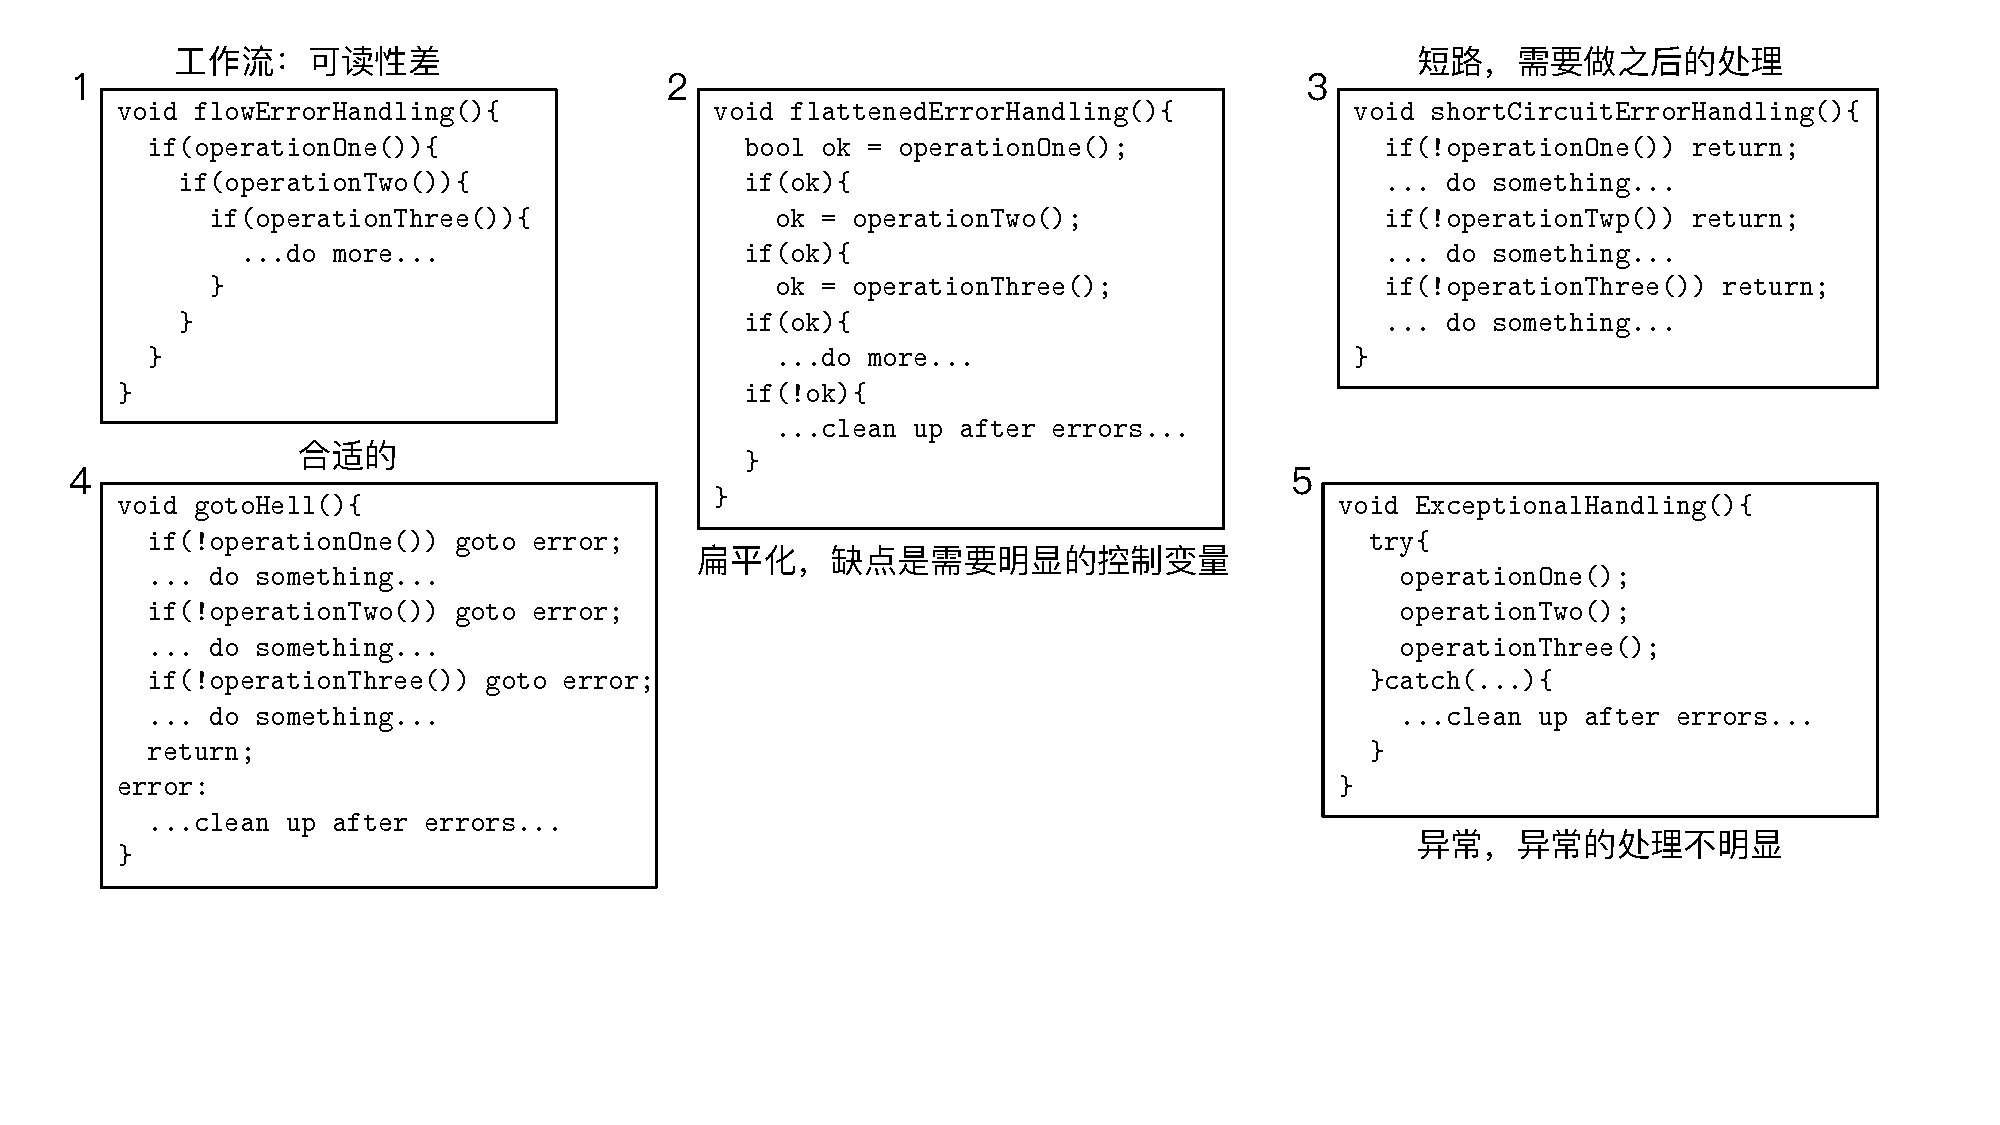
\includegraphics[width=0.95\textwidth]{images/错误处理代码示例.pdf}
    \vspace{-1em}
\end{figure}

\subsubsection{错误信息编写}
需要由用户清理错误时
\vspace{-0.8em}
\begin{multicols}{2}
\begin{itemize}
    \item 以用户期望的方式呈现信息
    \item 确保用户能够理解错误信息
    \item 不要呈现毫无意义的错误代码
    \item 将后果严重的错误与仅仅是警告区分开来
    \item 提示用户每种选择可能的后果后再提出问题
\end{itemize}
\end{multicols}
\vspace{-1em}

\subsection{异常}
异常是把代码中的错误或异常事件传递给调用方代码的一种特殊手段
\begin{itemize}
    \item 当遇到意料之外的情况,但不知道该如何处理时,可以抛出一个异常
    \item 同继承一样,谨慎使用可降低复杂度
\end{itemize}

异常处理的基本结构:
\begin{itemize}
    \item 子程序使用throw抛出一个异常对象
    \item 被调用链上层其他子程序的try-catch语句捕获
\end{itemize}

支持几种流行的编程语言的表达式
\vspace{-0.5em}
\begin{spacing}{1.2}
\centering
    \begin{longtable}{|m{3.3cm}<{\centering}|m{4.5cm}<{\centering}|m{3cm}<{\centering}|m{3cm}<{\centering}|}
        \hline
        \textbf{跟异常相关的特性}       & \textbf{C++}                                                                                                                                     & \textbf{Java}                                                                                              & \textbf{Visual Basic}        \\ \hline
    支持try-catch 语句          & 支持                                                                                                                                               & 支持                                                                                                         & 支持                           \\ \hline
    支持 try-catch-finally 语句 & 不支持                                                                                                                                              & 支持                                                                                                         & 支持                           \\ \hline
    能抛出什么                   & \verb|std::exception|\;对象或\sverb|std::exception|\;派生类的对象;对象指针;对象引用;string 或 int 等数据类型 & \verb|Exception|\;对象或\sverb|Exception|\;派生类的对象 & \verb|Exception|\;对象或\sverb|Exception|\;派生类的对象 \\ \hline
    未捕获的异常所造成的影响            & 调用\sverb|std::unexpected()|\;函数,该函数在默认情况下将调用\sverb|std::terminate()|,而这一函数在默认情况下又将调用\sverb|abort()|                                                                       & 如果是一个“受检异常”(checked exception)则终止正在执行的线程;如果是“运行时异常”(runtime exception)则不产生任何影响                             & 终止执行程序                       \\ \hline
    必须在类的接口中定义可能会拋出的异常      & 否                                                                                                                                                & 是                                                                                                          & 否                            \\ \hline
    必须在类的接口中定义可能会捕获的异常      & 否                                                                                                                                                & 是                                                                                                          & 否                            \\ \hline
    \end{longtable}
\end{spacing}
\vspace{-1em}

\vspace{-0.5em}
\begin{shaded}
{\kaishu 为何C++不提供“\verb|finally|”结构?}\\
因为C++提供了另一种机制,完全可以取代\sverb|finally|,而且这种机制几乎总要比\sverb|finally|\;工作得更好,就是“资源分配即初始化”(Resource Acquisition Is Initialization, RAII)。其基本的想法是,用一个局部对象来封装一个资源,这样一来局部对象的析构函数就可以自动释放资源。这样,程序员就不会“忘记释放资源”了。
\end{shaded}
\vspace{-1em}

\subsubsection{异常处理实例}
\begin{lstlisting}
try{
    statement1;  // Suppose no exceptions in the statements
    statement2;  // Suppose an exception of type Exception1 is thrown in statement2
    statement3;
}catch(Exception1 ex) {
    handling ex;  // The exception is handled.
}catch(Exception2 ex){
    handling ex;  // Handling exception 
    throw ex;  // Rethrow the exception and control is transferred to the caller
}finally {
    finalStatements; // The final block is always executed
}
Next statement;  // Next statement in the method is executed
\end{lstlisting}

\subsubsection{异常处理使用建议}
\begin{itemize}[leftmargin=1em]
    \item[$\checkmark$] 用异常通知程序的其他部分,发生了不可忽略的错误
    \begin{itemize}
        \item 能提供一种无法被忽略的错误通知机制
        \item 消除了错误向外扩散的可能性
    \end{itemize}
    \item[$\checkmark$] 只有真正例外的情况下才抛出异常
    \begin{itemize}
        \item 仅在其他编码实践方法无法解决的情况下才使用异常(同断言类似,处理罕见且不该发生的情况)
        \item 会增加复杂度:调用子程序的代码需要了解被调用代码中可能会抛出的异常,弱化了封装性
    \end{itemize}
    \item[$\checkmark$] 不能用异常来推卸责任:可以在局部处理就在局部处理掉
    \item[$\checkmark$] 避免在构造函数和析构函数中抛出异常,除非你在同一地方把它们捕获:C++中,构造函数中的异常会造成资源泄露
    \item[$\checkmark$] 在恰当的抽象层次抛出异常:确保异常的抽象层次与子程序接口的抽象层次是一致的
    \begin{lstlisting}
// Java反例:抛出抽象层次不一致的异常的类
class Employee{
    public TaxId GetTaxld() throws EOFException {
    }
}
// 子程序的调用方代码不是与Employee类的代码耦合,而是与比Employee类层次更低的抛出EOFException异常的代码耦合起来了
    \end{lstlisting}
    改进方法:\verb|GetTaxId()|\;代码应抛回一个与其所在类的接口相一致的异常
    \begin{lstlisting}
// Java示例:一个在一致的抽象层次上抛出异常的类
class Employee{
    public TaxId GetTaxld() throws EmployeeDataNotAvailable {
    }
} 
// 在设计上需要增加EmployeeDataNotAvailable异常类型,并将更底层的EOFException异常映射为该异常类型
    \end{lstlisting}
    \item[$\checkmark$] 在异常消息中加入关于导致异常发生的全部信息:确保消息中含有为理解异常抛出原因所需的信息,如数组下标错误
    \item[$\checkmark$] 避免使用空的catch语句:意味着try或catch里的代码不正确
    \begin{lstlisting}
try {
    // lots of code
} catch ( AnException exception ) {
    LogError("Unexpected exception");
} 
    \end{lstlisting}
    \item[$\checkmark$] 了解所用函数库可能抛出的异常
    \begin{itemize}
        \item 未能捕获由函数库抛出的异常可导致程序崩溃
        \item 可通过编写原型代码来演练该函数库
    \end{itemize}
    \item[$\checkmark$] 把项目中对异常的使用标准化
    \begin{itemize}
        \item 当抛出多种类型的异常,如对象、数据及指针的话,则考虑建立一个标准
        \item 创建项目的特定异常类:构造自己的异常类继承体系
        \item 规定哪些异常在局部处理,哪些不在局部处理
        \item 规定是否可以在构造或析构函数处理异常
        \item 确定是否要使用集中的异常报告机制
    \end{itemize}
    \item[$\checkmark$] 考虑创建一个集中的异常报告机制
    \item[$\checkmark$] 考虑异常的替换方案
    \begin{itemize}
        \item 不要因为编程语言提供了异常而使用它:“深入一种语言去编程”
        \item 应自始至终考虑各种各样的错误处理机制
        \item 思考是否真的需要处理异常
    \end{itemize}
    \begin{lstlisting}
try {
    System.out.println(refVar.toString());
} catch (NullPointerException ex){
    System.out.println("refVar is null");
}

if (refVar != null)
    System.out.println(refVar.toString());
else
    System.out.println("refVar is null");
    \end{lstlisting}
\end{itemize}

\subsection{通过隔栏包容错误}
\begin{itemize}
    \item 以防御式编程为目的而进行隔离的一种方法
    \item 把某些接口选定为“安全”区域的边界,对穿越安全区域边界的数据进行合法性校验
    \item 隔栏可以将检验工作集中在特定的模块中,从而降低其它部分采用防御式编程的成本
\end{itemize}

\begin{figure}[H]
    \vspace{-0.5em}
	\centering
	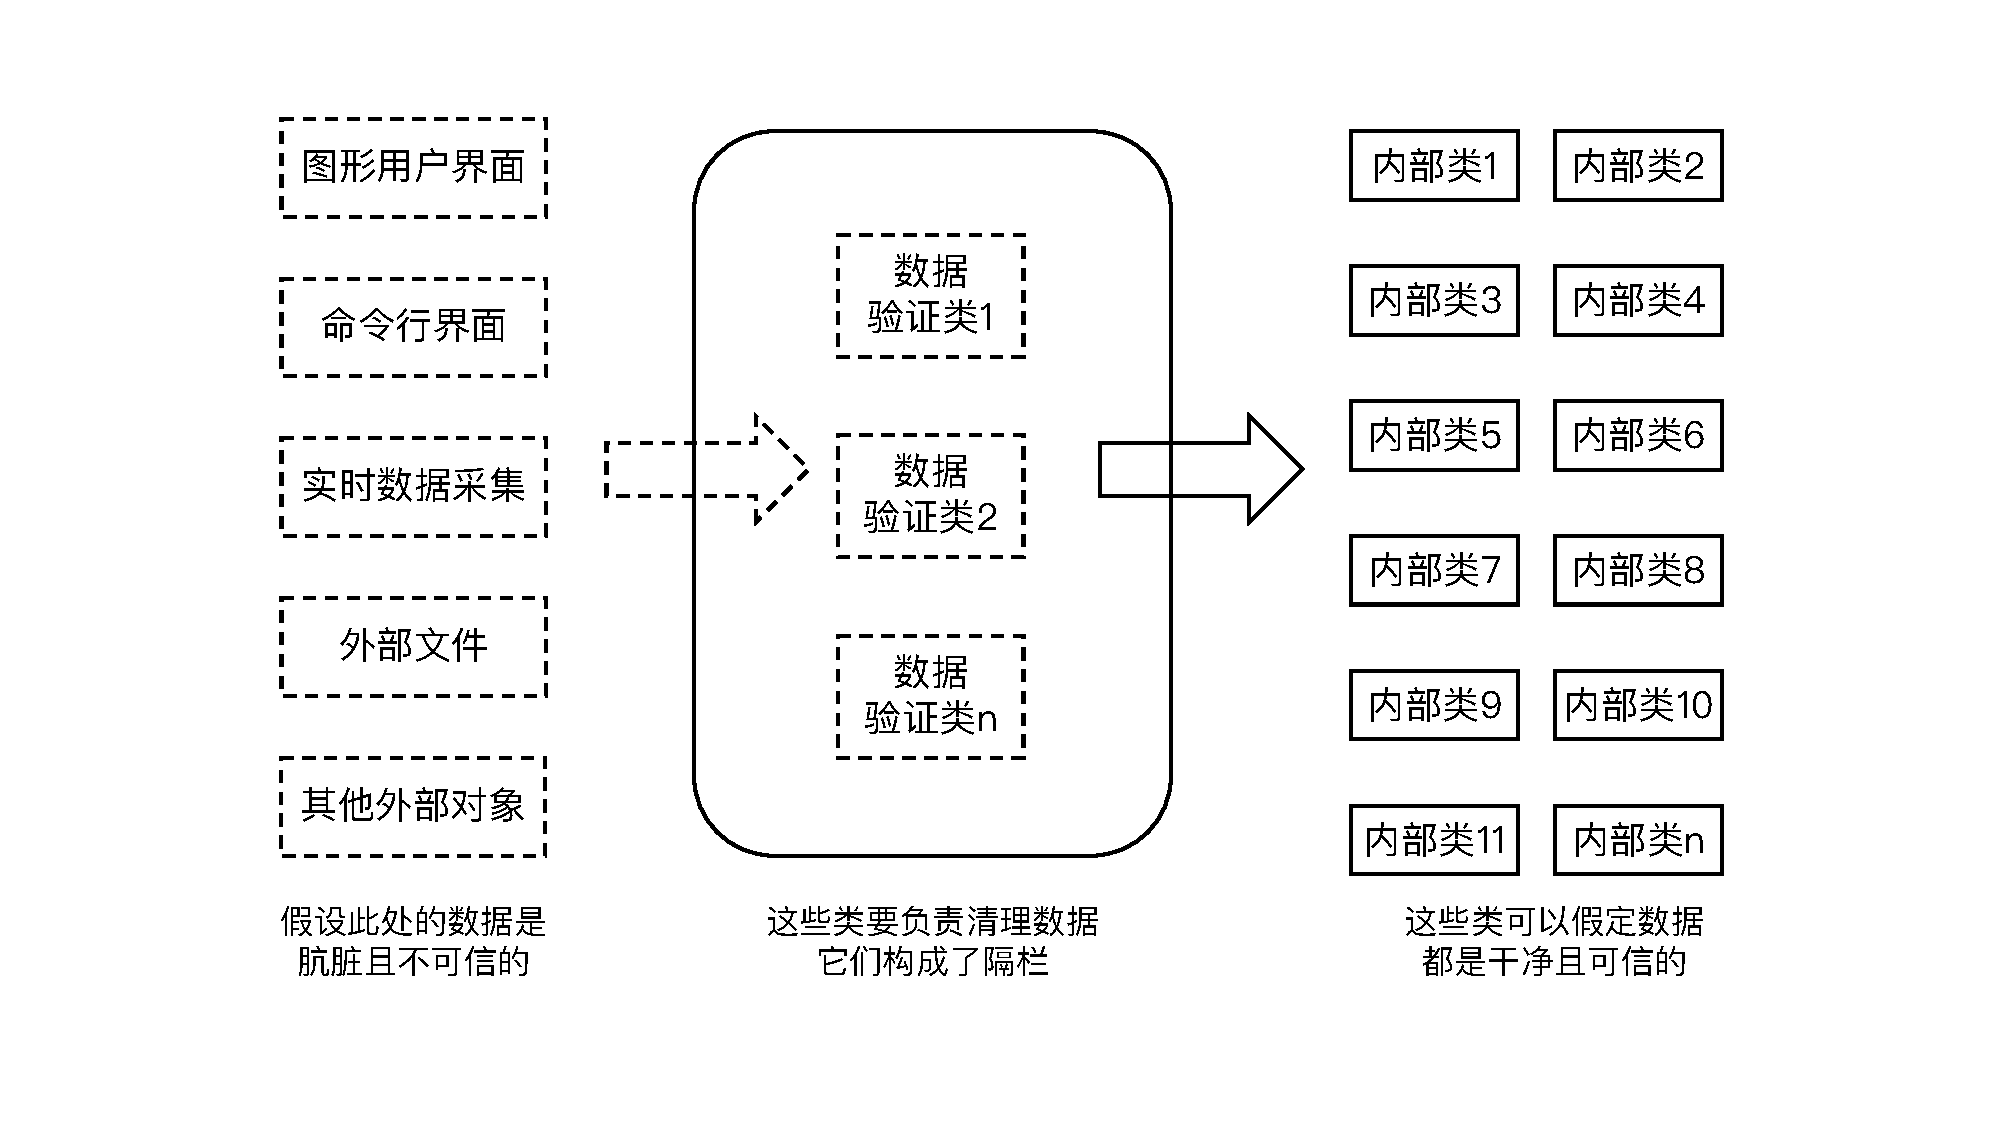
\includegraphics[width=0.6\textwidth]{images/通过隔栏包容错误.pdf}
    \vspace{-1em}
\end{figure}

在输入数据时将其转换为恰当的类型
\begin{itemize}
    \item 输入数据通常是字符串或数字
    \item 有时映射为“是”、“否”等布尔变量,有时是枚举变量
    \item 程序中长时间传递类型不明的数据,会增加程序的复杂度和崩溃的可能性,应该在输入数据后立即将其转换到恰当的类型
\end{itemize}

隔栏与断言的区别
\begin{itemize}
    \item 隔栏的使用使断言和错误处理有了清晰的区分
    \item 隔栏部分包含了“脏数据”:隔栏外部的程序应该使用错误处理技术,在那里对数据做任何的假定都是不安全的。
    \item 通过隔离部分之后的是“干净数据”
    \begin{itemize}
        \item 隔栏内部的程序就应使用断言技术,因为传进来的数据应该己在通过隔栏时被清理过了
        \item 隔栏内子程序出现错误数据,就是程序里的问题
    \end{itemize}
\end{itemize}

\subsection{辅助调试的代码}
防御式编程的另一重要方面是使用调试助手(辅助调试的代码),从而帮助快速检测错误
\begin{itemize}
    \item 误区: 产品级软件的种种限制也适用于开发中的软件,如性能、资源
    \item 正确的认识:应该在开发期间牺牲一些速度和资源,从而换取可以让开发更顺畅的内置工具
    \item 应该尽早地引入辅助调试的代码
\end{itemize}

\subsubsection{进攻式编程}
进攻式编程是主动暴露可能出现错误的态度:在开发阶段让它显现出来,而在产品代码运行时让它能够自我恢复

常用的进攻式编程方法
\begin{itemize}
    \item 确保断言语句使程序终止运行
    \item 完全填充分配到的所有内存
    \item 完全填充己分配到的所有文件或流
    \item 确保每一个case 语句中的default分支或else分支都能产生严重错误(如终止程序)
    \item 在删除一个对象之前把它填满垃圾数据
    \item 让程序把错误日志文件用电子邮件发给你
\end{itemize}

\subsubsection{移除辅助调试代码的方法}
辅助调试的代码会使软件的体积变得庞大且速度变慢,可以使用类似ant和make这样的版本控制工具和make工具
\begin{itemize}
    \item 在开发模式下,你可以让make工具把所有的调试代码都包含进来一起编译
    \item 在产品模式下,又可以让make工具把那些你不希望包含在商用版本中的调试代码排除在外
\end{itemize}

移除辅助调试代码的方法有使用内置的预处理器和使用调试存根

\textbf{使用内置的预处理器}:以用编译器开关来包含或排除调试用的代码
\begin{lstlisting}
#define DEBUG
#if defined(DEBUG)
#define DebugCode(code-fragment) {code-fragment}
#else
#define DebugCode(code_fragment)
#endif
...
DebugCode(
    statement 1;
    statement 2;
    ...
    statement n;
);
...
\end{lstlisting}

\textbf{使用调试存根}debugging stubs:开发代码中调用某子程序进行调试检查,产品代码中使用桩子程序替换它
\begin{figure}[H]
    \vspace{-0.5em}
	\centering
	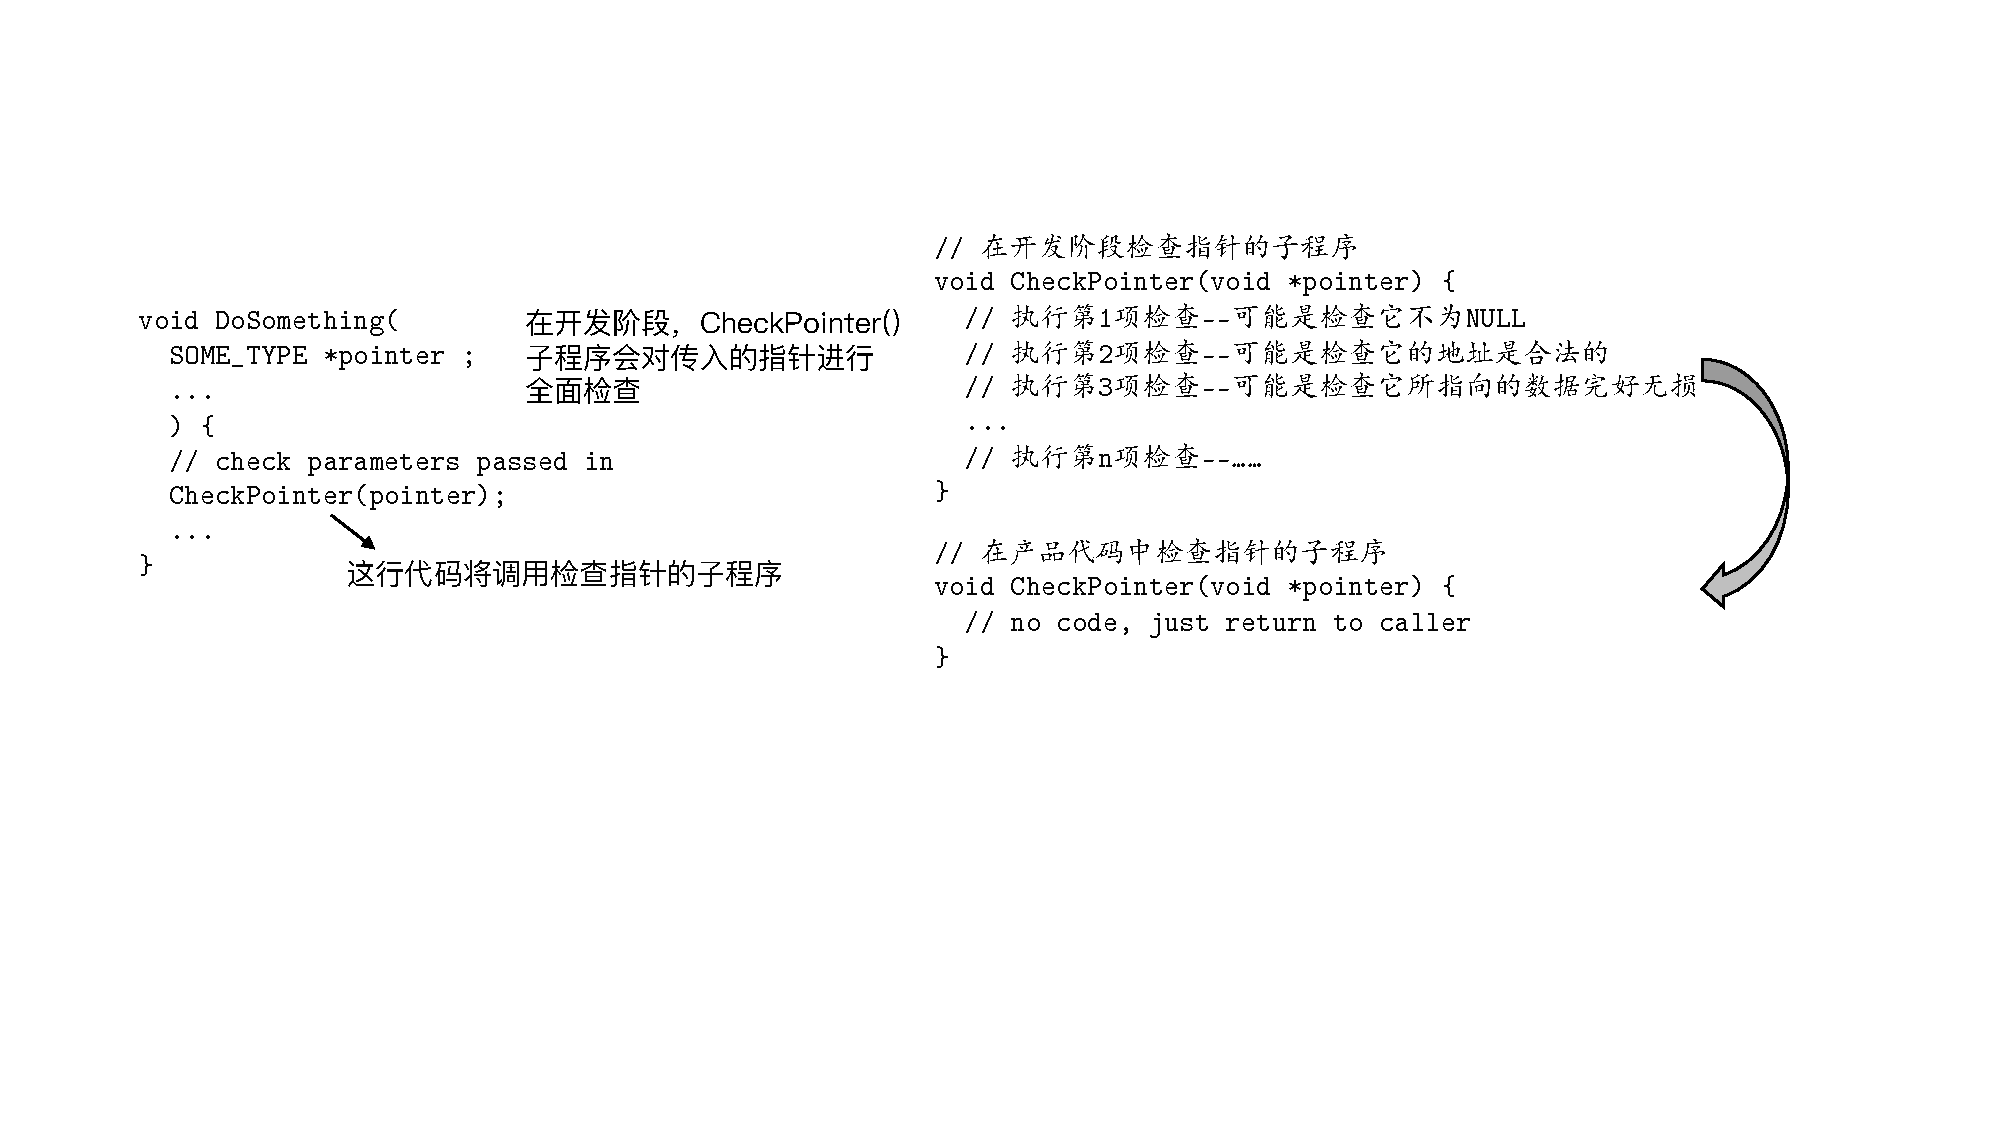
\includegraphics[width=\textwidth]{images/使用调试存根.pdf}
    \vspace{-1em}
\end{figure}


\subsection{对防御式编程的防御式态度}
产品代码中应该保留多少防御式代码
\begin{itemize}
    \item 开发阶段:显示出的错误越多越好,引入很多防御代码
    \item 发布阶段:希望错误尽可能偃旗息鼓,不要影响代码执行
    \item 保留那些检查重要错误的代码
    \item 去掉检查细微错误的代码
    \item 去掉可以导致程序硬性崩溃的代码:用户无法保存必要数据
    \item 保留可以让程序稳妥地崩溃的代码:用于诊断潜在的严重错误
    \item 为你的技术支持人员记录错误信息
    \item 确认留在代码中的错误消息是友好的:“发生了内部错误,可联系XX”
\end{itemize}

\vspace{-0.8em}
\begin{multicols}{2}
    过度的防御式编程也会引起问题
\begin{itemize}
    \item 程序会变得臃肿而缓慢
    \item 增加了软件的复杂度
    \item 防御式代码同样会有缺陷
\end{itemize}

正确的态度
\begin{itemize}
    \item 采用防御的姿态
    \item 考虑好什么地方进行防御
    \item 因地制宜地调整防御式编程的优先级
\end{itemize}
\end{multicols}
\vspace{-1em}



